%! Author = Saeid Yazdani
%! Date = 5/14/2023


\chapter{Time-Variant Based \acs{DPS}}
\label{ch:proposed-control-loop}

In this chapter, we will describe in detail the implementation of a \ac{DPS}
based on the proposed \emph{Time-Variant} approach for control loop and output
regulation.

Throughout this text, the \ac{DPS} will be referred to by its nickname,
\ac{HVS}.
One of the key advantages of this system is its ability to provide a wide range
of voltage and current levels, making it suitable not only for low-power devices
like microcontrollers and logic ICs but also for high-power applications
while maintaining acceptable accuracy and precision at all ranges.


\section{System Specification}
\label{sec:ch-sys-spec-intro}

Comprehensive specifications have been defined for the proposed \ac{DPS} system.
The \ac{HVS} will be a Four-Quadrant (\autoref{fig:fourd-quadrant-psu-overview})
bipolar \ac{SMU} capable of sourcing, sinking and measuring negative and
positive voltages and currents according to standard features expected from
a laboratory-grade power supply with specifications listed in
\autoref{tab:hvs-measurement-nominal-accuracy}.

\begin{figure}[h]
    \centering
    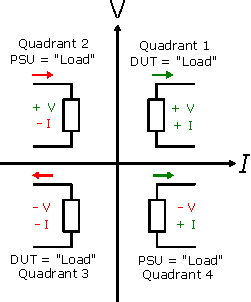
\includegraphics[scale=1.05]
    {figures/four-quadrant-psu-coordinates}
    \caption[Four-Quadrant Power Supply]{Overview of output directions and
    modes of a four-quadrant power supply.}
    \label{fig:fourd-quadrant-psu-overview}
\end{figure}

The \ac{HVS} integrates standard features and safety measures
that are expected from a power supply for highly sophisticated \acp{DUT}:
We guarantee safe and reliable operation both for the operator and
overload-sensitive \acp{DUT}.
Thanks to a digital controller, many safety features can be realized in software
rather than in hardware.

\begin{table}[h!] % [h1] Causes the table be positioned within the text
    \centering
    \begin{tabular}{l|c|c}
        \toprule
        \textbf{Parameter} & \textbf{Range}                            & \textbf{Accuracy} \\
        \midrule
        \midrule
        Source Voltage     & \SI{100}{\milli\volt} to \SI{1000}{\volt} & 0.05\%            \\

        Measure Voltage    & \SI{1000}{\volt}                          & 0.2\%             \\
        \midrule
        Measure Current    & \SI{10}{\nano\ampere}                     & 1\%               \\

        \text{  } & \SI{100}{\nano\ampere} to \SI{10}{\milli\ampere}
        & 0.05\% \\

        \text{  } & \SI{100}{\milli\ampere} to \SI{1}{\ampere}
        & 0.1\% \\

        \text{  }            & \SI{10}{\ampere}                          & 0.2\%

    \end{tabular}
    \caption{\acs{HVS} Output and Measurement expected accuracy levels}
    \label{tab:hvs-measurement-nominal-accuracy}
\end{table}

\ac{OCP} and \ac{OVP} can be realized in software, since the system has
near-instantaneous awareness of the actual output levels and can constantly compare
the required voltage and current levels set by the application with
pre-defined limits.

If for any reason a \ac{DUT} starts to draw more power than intended,
the digital controller can immediately detect and react to that load condition.
For absolute safety, the \ac{HVS} will incorporate a hardware
limiting circuit per output range, called \emph{static}
protection.


\section{System overview}
\label{sec:system-overview}

The \ac{HVS} is built as a modular system as presented in
\autoref{fig:hvs-hvs-controller-board-diagram} and contains the following
main blocks:

\begin{itemize}[topsep=8pt,itemsep=4pt,partopsep=4pt, parsep=4pt]

    \item \textbf{Controller Board:} Tasked with system management and control
    which contains the following items:
    \begin{itemize}[topsep=8pt,itemsep=4pt,partopsep=4pt, parsep=4pt]
        \item Microcontroller: communication and control, mode configuration,
        power-supply settings, test controller.
        \item FPGA: digital control loop, ADC/DAC interfaces, measurement
        functions, clamping control, averaging and sampling functions.
        \item \acs{ADC} and \acs{DAC} chips.
    \end{itemize}

    \item \textbf{Amplifier Board:} A high-voltage high-current four-quadrant
    amplifier is the driving force. The amplifier is a 3-stage design with:
    \begin{itemize}[topsep=8pt,itemsep=4pt,partopsep=4pt, parsep=4pt]
        \item {high-precision pre-amp for high loop gain (\SI{\pm10}{\volt})}
        \item {high-voltage amplifier (\SI{\pm350}{\volt})}
        \item {high-current booster stage (\SI{\pm10}{\ampere} pulsed or \SI{\pm2}{\ampere} continuous)}
    \end{itemize}

    \item \textbf{Frontend:} Is the final stage of the output and
    contains output connectors and pin relays as well as buffer amplifiers for
    sampling the output to be redirected to the control processor for feedback
    calculations.
    \begin{itemize}[topsep=8pt,itemsep=4pt,partopsep=4pt, parsep=4pt]
        \item {Programmable shunt resistor network for current measurements,}
        \item {Programmable voltage divider network for voltage measurements.}
    \end{itemize}

    \item \textbf{Current Limiter:} Contains an array of resistors for limiting
    output currents in emergency caes to safe values specified in test programs.

    \item \textbf{Main Switching Supply:} Tracking rail \acs{DC}/\acs{DC}
    converters for the power amplifier to minimize internal losses:

    \begin{itemize}[topsep=8pt,itemsep=4pt,partopsep=4pt, parsep=4pt]
        \item
        A switching supply sets all rails to \( \lvert V_{OUT} \rvert +
        \lvert V_{DROP} \rvert \), where \( V_{DROP} \) is the minimum rail
        overhead to guarantee perfect amplifier operation.

        \item
        By using a \acs{FET}-bases source follower circuit the expected votlage
        drop will be small as a \acs{FET}-based source follower
        ciruit the minimum voltage drop will be larger than
        \( R_{\text{DS(ON)}} \times I_{LOAD} \)
        since the channel resistances of power \acs{FET}s are in the range of a
        few \SI{}{\milli\ohm}.
    \end{itemize}

    \item \textbf{Monitor Board:} A set of buffer amplifiers to allow
    for the monitoring the output of the system in analog fashion (e.g. connect to
    and oscilloscope) for observation or debugging. The board contains:
    \begin{itemize}[topsep=8pt,itemsep=4pt,partopsep=4pt, parsep=4pt]
        \item {Normalized analog monitor outputs, }
        \item {Modulation input for external analogue control.}
    \end{itemize}

\end{itemize}

\begin{figure}[h]
    \centering
    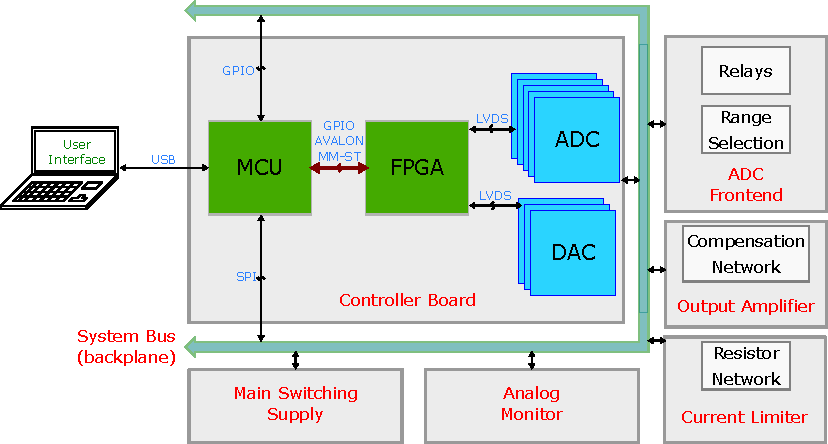
\includegraphics[width=\textwidth]
    {figures/hvs/digital-board-connections}
    \caption[HVS Control board]{Control board in HVS contains the digital
    control loop and an interface between the user and analog front end}
    \label{fig:hvs-hvs-controller-board-diagram}
\end{figure}

The control loop algorithm is realized on the FPGA which is interfaced through
\ac{LVDS} to high-speed \acs{ADC}s and
\acs{DAC}s which read voltages and currents on multiple nodes of the
feedback path and drive output stage amplifiers respectively.

Communication between FPGA and microcontroller is implemented using an
AVALON-like\footnote{
    The Avalon® Interface is a bus protocol used in FPGA designs to facilitate
    communication between components and is designed by Altera Corporation, which is
    now part of Intel Corporation.} bus for fast parallel communication betweenthe
two units.
All the settings and variables associated with the control loop operation are in
registers defined in the \ac{FPGA}.

The \ac{MCU} and high-voltage supplies, current limiter
board and gain setting switches on the analog front-end (\ac{ADC})
communicate via an \acs{SPI} interface.

The communication with the outside world comes through a \acs{USB} interface
and users or other instruments (e.g. \acs{ATE} test control software) will be
able to operate and manage the system using a \acs{GUI} or through a
dedicated \ac{API}.
%%%%%%%%%%%%%%%%%%%%%%%%%%%%%%%%%%%%%%%%%%%%%%%%%%%%%%%%%%%%%%%%%%%%%%%%%%%%%%%%


\section{\acs{FPGA} and \acs{MCU} Structures}
\label{sec:fpga-mcu-structures}

The design is implemented on an Intel Cyclone V \ac{FPGA}.
The \ac{FPGA} is responsible for on-the-fly compensation adaptation,
output signal supervision on several channels (safety features), and the
loop-back d-to-a converters.

Three clocked register banks based on D flip-flops are implemented in the FPGA
for storing configuration settings such as output management,
scaling of \ac{DAC} and \ac{ADC} depending on the active selected range, and
special functions such as custom waveform generation by the \ac{HVS}.
These registers are read and written via the parallel Avalon® bus by
the MCU.

The Avalon bus is implemented as a master/slave \emph{Memory Mapped} (MM)
interface where the \ac{MCU} as the master can read from or write to specific
memory-mapped addresses in the \ac{FPGA} (slave).
This bus implementation supports operations like read, write, and
burst transfers (e.g. for measurement readouts).

The physical implementation of this bus uses two complete ports of the
\ac{MCU} (16 I/O pins each), for address and data in addition to extra I/O pins
from another \ac{MCU} port dedicated to data transfer control signals such as
read or write requests.

\begin{figure}[h]
    \centering
    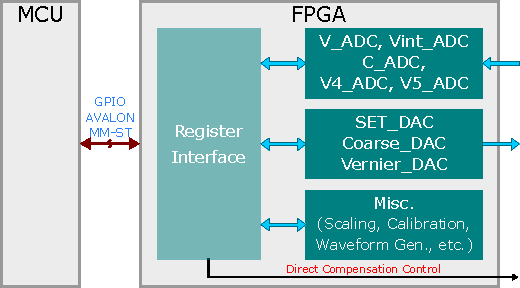
\includegraphics[width=0.8\textwidth]
    {figures/design-realization/fpga-and-mcu-block}
    \caption[\acs{FPGA} and \acs{MCU} Connection Diagram]{
        Block diagram of \acs{FPGA} and \acs{MCU} and their internal
        connections.
    }
    \label{fig:fpga-mcu-diagram}
\end{figure}

This implementation allows the bus to be used in \emph{Streaming} (ST)
mode, if required.
In \emph{ST} mode, the focus will be on high-throughput, low-latency data
transfer for efficient streaming.

The \ac{MCU} sets all static and dynamic values such as calibration data,
range-selection and output relays at start-up and during runtime.

The list of registers and their description is presented in
\hyperref[sec:hvs-fpga-register-map]{Appendix A}.

%%%%%%%%%%%%%%%%%%%%%%%%%%%%%%%%%%%%%%%%%%%%%%%%%%%%%%%%%%%%%%%%%%%%%%%%%%%%%%%%
%! Author = Saeid Yazdani
%! Date = 8/10/2024


\section{Control loop details}
\label{sec:loopdetails}

\autoref{fig:loop-algo} shows the high-level block diagram of the control loop
components.

The control loop algorithm starts from data that are generated from analog
signals by the \ac{ADC} modules.
Data correction for \emph{offset} and full-scale range gain settings precedes
range scaling to the control loop's SET DAC.

The \acs{FPGA} manages \emph{Compensation}, \emph{\acs{DAC}} and
\emph{\acs{ADC}} blocks and controls all the dynamic operations:

\begin{itemize}[topsep=8pt,itemsep=4pt,partopsep=4pt, parsep=4pt]
    \item Repetitive reading of all ADC values coming from five ADC chips
    through the \ac{LVDS} interface.

    \item Calculation of control loop signals sent to the control loop DAC for:
    \begin{itemize}[topsep=8pt,itemsep=4pt,partopsep=4pt, parsep=4pt]
        \item Offset correction,
        \item \acs{FSR} Scaling, over-range limitation (clamp function),
        \item Data correction and re-scaling for the DAC \acs{FSR}
    \end{itemize}

    \item Transfer and receive runtime data to and from the registers to
    \ac{MCU} using the parallel bus.
    \item Output of the compensation data (dynamic loop control) as pre-defined
    by the \ac{MCU}.

\end{itemize}

In any control loop, we compensate the control amplifier's \emph{SET} input
signal such that the output signal reaches the \emph{target} value.
We get a \emph{zero} input signal only if the amplifier’s gain is infinity – in
a practical approach we use an input signal of $V_{OUT}$ and \emph {GAIN} at the
summing point – the lower the gain the higher the summing node signal.

Output current is measured using shunt resistors for given output ranges
in a high-side current measurement configuration.
The current sense signal is transferred to the control system via optically
isolated data communication lines.

If the control input is switched to the \emph{Current Sense} signal we get a
current source and the voltage \emph{clamp} is activated.

\begin{figure}[htbp]
    \centering
    \printfitgraphics[0.62\textheight]{figures/design-realization/hvs-control-overview}
    \caption[\acs{FPGA} Control Loop Diagram]{
        High-level block diagram of the control loop components inside
        the FPGA.
    }
    \label{fig:loop-algo}
\end{figure}

\subsection{Input Processing}
\label{subsec:input-processing}

\autoref{fig:fpga-input-block_fpga_input_processing} shows the flow of
data for processing control loop output value inside the FPGA.
An optional moving average window and an inverter stage are provisioned.
Data acceptance can be paused to inject test data to debug the control loop.

\begin{figure}[h]
    \centering
    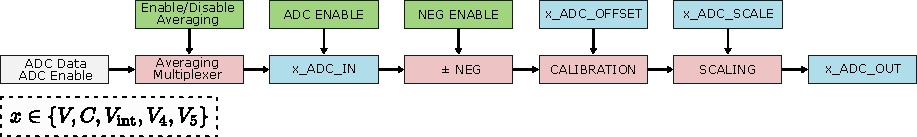
\includegraphics[width=1\textwidth]
    {figures/design-realization/fpga_input_processing}
    \caption[FPGA Input processing]{
        Overview of data flow for processing loop variables by the FPGA.
    }
    \label{fig:fpga-input-block_fpga_input_processing}
\end{figure}

There are five ADC blocks with 4 dedicated registers assigned to each.
These registers (5x4) associated with \ac{ADC} chips are mapped to address
ranges \texttt{0x00} to \texttt{0x13}.
The input blocks are performing the following tasks during runtime:

\begin{itemize}[topsep=8pt,itemsep=4pt,partopsep=4pt, parsep=4pt]
    \item{Continuous reading of all ADC values (five ADC)}
    \item{Calculation of appropriate control loop settings}
    \item {Continuous output of DAC values}
\end{itemize}

All measured values from the ADC are corrected in the first step according
to individual correction data, scaled to the target range of the DAC, and
then transferred to the DAC for proper control loop operation.
All ADC values are stored in a \ac{DPRAM} buffer on the FPGA for further
analysis.

A moving average window is available, data acceptance can be stopped for
injecting test data, and an inverter stage is available.

\subsection{Output Processing}
\label{subsec:output-processing}


The input data for the loop's set DAC are combined data from \emph{SET} and
\emph{VERNIER} (alternatively used for \emph{offset}) and \emph{COARSE}.
All data are scaled (\texttt{1.0} = \texttt{0x1000}) and offset (signed integer) to
adjust the number representations.
The 12 DAC registers (3x4) are mapped to address \texttt{0x14} to
\texttt{0x1F}.

\subsection{Calibration of \acs{DAC} and \acs{ADC}}
\label{subsec:dac-and-adc-calibration}

The physical components of the system especially in the \acs{ADC} and \acs{DAC}
blocks can drift as a result of aging and environmental effects such as
temperature and humidity.
Therefore, range adjustments and offset corrections are necessary to compensate for
these variations to ensure the system maintains accuracy and reliability.
Range adjustment is necessary to prevent the output from exceeding the
operational limits of the components of the system.
\autoref{table:fsr-range-adjustments} shows the provisioned values for range
adjustment.

\begin{table}[h]
    \centering
    \begin{tabular}{c|c|c}
%        \hline
        \multicolumn{3}{c}{\small \textbf{Range Adjustment for \acs{DAC} and \acs{ADC}}} \\ \cline{1-3}
        \texttt{0x7FFF} & maximum value     & \texttt{0xFFFF} \\ \hline
        \texttt{0x0000} & zero              & \texttt{0x8000} \\ \hline
        \texttt{0x8000} & - (maximum value) & \texttt{0x0000} \\ \hline
    \end{tabular}
    \caption[\acs{DAC} and \acs{ADC} Range Adjustments]{
        Range adjustments for all DAC and ADC modules ensure that the input and
        output signals are appropriately scaled to match their \acs{FSR}.
    }
    \label{table:fsr-range-adjustments}
\end{table}

The DAC and ADC drifts are corrected via dedicated offset \emph{offset}
registers.
For example, an analog \SI{0}{\volt} should be generated for a
\acs{DAC} value of \texttt{0x0000}.
But instead, we may get \SI{4}{\milli\volt} of deviation.
This deviation will be the calibration value equal to
\texttt{0xFFF1} (\SI{-4}{\milli\volt}) for this particular DAC value.
The output is then corrected to \SI{0}{\volt}.
ADC modules in the system also may show a slight offset resulting in small
non-zero values such as \texttt{0x0008} to be generated for a \SI{0}{\volt}
input, hence it is also necessary to calibrate and correct the ADC values.

The calibration procedure can be done for every bit of the \acs{FSR} or with a
skip factor and normalization over the skipped range with a tradeoff
between precision and execution time.
Dedicated calibration blocks in the \acs{FPGA}
are tasked to correct DAC and ADC values using the offset factors
saved in calibration \ac{LUT} as shown in \autoref{fig:dac-adc-calib}.

\begin{figure}[h]
    \centering
    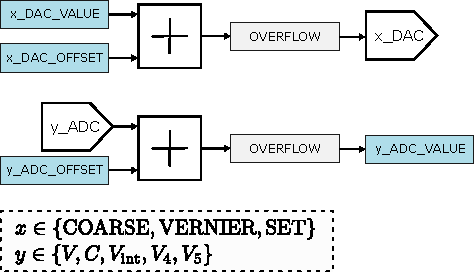
\includegraphics[width=0.7\textwidth]
    {figures/design-realization/adc-and-dac-calibration}
    \caption[Calibration of ADC and DAC]{
        Calibration blocks for \acs{DAC} (top) and \acs{ADC} (bottom).
    }
    \label{fig:dac-adc-calib}
\end{figure}

\subsection{Scaling \acs{ADC} and \acs{DAC} values}
\label{subsec:scaling-adc-dac}

At different voltage and current ranges, the adjusted range from ADC to DAC
blocks may not align correctly due to:

\begin{itemize}[topsep=8pt,itemsep=4pt,partopsep=4pt, parsep=4pt]
    \item \textbf{Range Mismatch:}
    The ADC might be converting the input signal to a digital value over a
    different range than the DAC expects.

    \item \textbf{Gain Differences:}
    If the gain applied by the ADC is different from that expected by the DAC,
    the digital data might not represent the analog signal accurately when
    converted back by the DAC.

\end{itemize}

In such cases, scaling is a necessary step if the measured and offset-corrected
ADC data does not match the output of the DAC.
The scaling operation is done by multiplying ADC values by a dedicated block
inside the FPGA as shown in \autoref{fig:dac-adc-scaling}.

\begin{figure}[h]
    \centering
    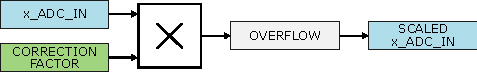
\includegraphics[width=0.7\textwidth]
    {figures/design-realization/fpga-adc-dac-scaling}
    \caption[ADC-DAC Scaling]{
        Block diagram of the scaling operation inside the FPGA.
    }
    \label{fig:dac-adc-scaling}
\end{figure}

The scale factor is generated through reference data collection and maintenance
procedures that involve supplying test signals into ADC chips and recording
their outputs.
These ADC outputs will be sent to corresponding DACs and the resulting analog
outputs will be recorded.
The scale factor for a given bit or range of bits is then calculated
according to \autoref{eq:scale-factor}.

\begin{equation}
    \label{eq:scale-factor}
    \text{Scale Factor} = \frac{\text{Expected Output}}{\text{Actual Output}}
\end{equation}

When the voltage ADC or the current ADC reaches their \acs{FSR} limits, we need
to lower the set point voltage until the ADC readings return to non-limited
values.
Therefore, a \emph{re-scaling} or \emph{scale-limiting} block is necessary to
prevent clipping.

\begin{figure}[h]
    \centering
    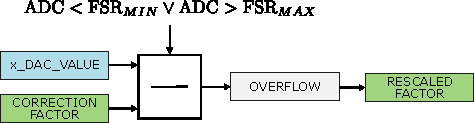
\includegraphics[width=0.7\textwidth]
    {figures/design-realization/adc-rescaling}
    \caption[Scale Limiter]{
        Block diagram of scale-limiter inside the \ac{FPGA}.
    }
    \label{fig:scale-limiter}
\end{figure}

\subsection{\acs{ADC} Averaging}
\label{subsec:adc-averaging}

ADC readings can be affected by random electrical noise, which causes small
fluctuations in the output.
Averaging multiple samples helps smooth out these fluctuations and yield
accurate and stable representation of the signal.

As stated before, an optional averaging block is provisioned in the \ac{FPGA}
with configurable window sizes of 2, 4, 8, and 16 samples that can be enabled or
bypassed for faster response, as averaging will result in slower response time
and reduced temporal resolution, affecting the dynamic behavior of the system
especially in transient events.

The averaging operation is done in the FPGA by division operation over
the sum of selected data samples according to the window size as shown in
\autoref{fig:adc-averaging}.

\begin{figure}[h]
    \centering
    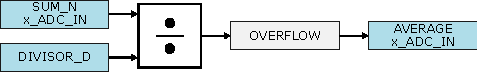
\includegraphics[width=0.7\textwidth]
    {figures/design-realization/fpga_averaging}
    \caption[ADC Value Averaging]{
        Block diagram of the averaging operation inside the FPGA.
    }
    \label{fig:adc-averaging}
\end{figure}

\subsection{RAM Analysis}
\label{subsec:ram-analysis}

The system stores $2^{16}$ ADC samples every time that a new SET DAC value has
been applied.
We can skip a pre-defined number of samples for storing using ACCESS\_CNT
registers individually per Voltage ADC and Current ADC dedicated registers.
This allows for the acquisition of different waveforms in current and voltage.
The microcontroller can read these data for further processing.


%%%%%%%%%%%%%%%%%%%%%%%%%%%%%%%%%%%%%%%%%%%%%%%%%%%%%%%%%%%%%%%%%%%%%%%%%%%%%%%%
%%%%%%%%%%%%%%%%%%%%%%%%%%%%%%%%%%%%%%%%%%%%%%%%%%%%%%%%%%%%%%%%%%%%%%%%%%%%%%%%
%! Author = Saeid Yazdani
%! Date = 8/15/2024


\section{Compensation Unit}
\label{sec:compensation-network}

The control loop can be characterized by frequency response on the output and
a compensation network is necessary for maintaining the stability, response
time, and performance of the feedback loop that regulates the output voltage or
current under various load conditions.

There are several ways to achieve the best-case compensation.
In the first approach, we don't change the amplifier's compensation during
the control loop calculations.
Instead, compensation is provided by an RC network and a set of electronic
relays, which help to optimize the control loop's behavior.
In the subsequent step, the compensation network can be adjusted on the fly,
leading to a more optimized step response.

\subsection{Static Compensation}
\label{subsec:static-compensation}

The two registers, PRECMP\_C (pre-amplifier compensation capacitor array) and
PRECMP\_R (pre-amplifier compensation resistor array), define the static
settings for compensation.
Additionally, there are PACMP\_C (power-amplifier compensation capacitor array)
and PACMP\_R (power-amplifier compensation resistor array) for extra
compensation of the power amplifier, even though the power amplifier may not
require variable compensation during runtime.
Clearing the CONFIG\_REG[14] bit enables online compensation.
In the initial approach, we maintain all compensation settings as constant
(the slowest version).
Static compensation can then be adjusted based on the results of the system
characterizations after production.

\subsection{Dynamic Compensation}
\label{subsec:dynamic-compensation}

Dynamic compensation involves modifying the compensation settings at
specific points in time and is the basis for the adaptive-predictive
compensation discussed in \autoref{subsec:time-variant-comp-network}.

For each timing event, we have a set of corresponding timing registers,
TIM\_0 to TIM\_7.
When the internal counter reaches the value set in the first timing register,
the corresponding compensation settings are applied.
This process continues sequentially through up to eight register sets.

By default, the dynamic compensation scheme is active and can be disabled by
clearing the CONFIG\_REG[14] bit (switch to static compensation mode).
The internal counter begins from zero, triggered by a signal when a new SET
value is generated (a short pulse to logic level 1, then immediately returning
to zero).

Dynamic compensation settings are designed to optimize the transition
times for output signals.
As the output signal approaches the target value, the initial rise time is
reduced, minimizing overshoot and ensuring a smooth entry into the tolerance
band.

\subsection{Compensation Control in the \acs{FPGA}}
\label{subsec:compensation-control-fpga}

The dynamic compensation system functions by selectively engaging and
disengaging arrays of resistors and capacitors.
Given that modifying the compensation network is a time-critical task,
the decision-making algorithm is implemented within the FPGA logic.
This implementation allows for timely control of the R/C arrays via
FPGA's GPIO pins, eliminating the need for \ac{MCU} and associated bus-access
overhead.

\autoref{tab:compensattion-registers-fpga} shows the dedicated registers
for controlling the compensation networks.

\begin{table}[h]
    \centering
    \resizebox{\linewidth}{!}{%
    \begin{tabular}{|>{\centering\arraybackslash}m{0.2\textwidth}|>{\centering\arraybackslash}m{0.2\textwidth}|>{\centering\arraybackslash}m{0.1\textwidth}|>{\centering\arraybackslash}m{0.05\textwidth}|>{\centering\arraybackslash}m{0.35\textwidth}|}
        \hline
        \text{Address (dec)} & \text{Address (hex)}            & \text{Bits} & \text{Type} & \text{Desciption}      \\
        \hline
        64 - 71              & \texttt{0x40} .. \texttt{0x47}  & 8           & RW          & Pre-amplifier 0 to 7   \\
        \hline
        72 - 79              & \texttt{0x48} .. \texttt{0x4F}  & 8           & RW          & Power Amplifier 0 to 7 \\
        \hline
        80 - 87              & \texttt{0x500} .. \texttt{0x57} & 8           & RW          & Timing 0 to 7          \\
        \hline
    \end{tabular}
    }
    \caption[Compensation Registers]{
        Compensation Registers in the \acs{FPGA}
    }
    \label{tab:compensattion-registers-fpga}
\end{table}


Each timing register specifies the exact moment when the values from the
compensation register are applied. When a new value is written, compensation
is initially set to its minimum.
An internal counter, starting from 0, continuously compares its value with the
timing registers 0 through 7.
When a match is found, the corresponding compensation setting is activated
by switching control relays using \acs{FPGA}'s \acs{GPIO} pins.
This procedure is depicted in \autoref{fig:compensation-apply-timing}
and \autoref{fig:compensation-arrangement}.

At system startup, the microcontroller is responsible for configuring all
settings and writing them into 24 registers.
These values are independent of the applied voltage and current ranges; they
must be fine-tuned during the characterization of \acs{HVS} after production.


\begin{figure}[t!]
    \centering
    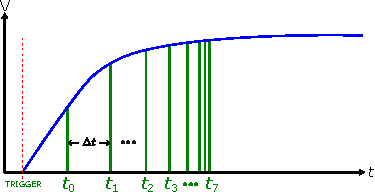
\includegraphics[width=0.6\textwidth]
    {figures/design-realization/compensation-apply-timing}
    \caption[Compensation Apply Timer]{
        The compensation network is set within 8 discrete steps.
        The timing between steps is customizable through TIM\_0 to TIM\_7 registers
        and a resolution of \SI{1}{\nano\second} is theoretically possible and is
        subject to the speed of analog switches used in the circuit.
        The reset values of timing registers are as follows:
        \SI{44.8}{\micro\second}, \SI{22.4}{\micro\second},
        \SI{11.2}{\micro\second}, \SI{5.6}{\micro\second},
        \SI{2.8}{\micro\second}, \SI{1.4}{\micro\second},
        \SI{0.7}{\micro\second}, \SI{0.4}{\micro\second}
    }
    \label{fig:compensation-apply-timing}
\end{figure}

\begin{figure}[t!]
    \centering
    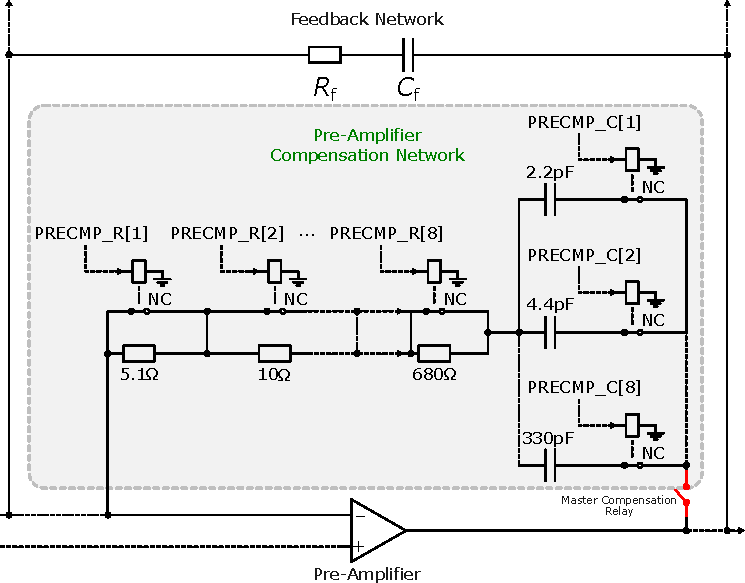
\includegraphics[width=0.9\textwidth]
    {figures/design-realization/compensation-arrangement}
    \caption[Pre-Amplifier Compensation Network]{
        Arrangement of series resistor-capacitor compensation network
        for the pre-amplifier (the power amplifier has a similar arrangement).
        A Master relay is used to enable/disable the network completely, based
        on configuration registers.
        Each component in the network has a dedicated \ac{NC} analog switch
        that is controlled by the \ac{FPGA}.
        A Wide range of R-C values can be achieved by series and parallel
        combination of the components in the network.
    }
    \label{fig:compensation-arrangement}
\end{figure}

The complete list of compensation network resistor and capacitor values
and their associated registers is given in
\hyperref[sec:compensation-network-values]{Appendix B}.

%%%%%%%%%%%%%%%%%%%%%%%%%%%%%%%%%%%%%%%%%%%%%%%%%%%%%%%%%%%%%%%%%%%%%%%%%%%%%%%%
